\section{Estado da Arte} \label{sec:fundaments}

Para o roteamento de fibras, é necessário pelo menos o entendimento básico de
dois temas: (1) a composição de elementos passivos das redes ópticas e (2)
algoritmos (no sentido de operações, otimização e tipos de problemas).

\subsection{Redes Ópticas}

Na teoria dos grafos, um grafo é uma estrutura composta por vértices ($V$)
(também chamados de nós) e arestas ($E$). A relação entre $V$ e $E$ é dado por
$G(V,E)$. Fazendo um paralelo com uma rede óptica, os vértices seriam as Caixas
de Emenda (CE) e as Caixas de Atendimento (CA) \cite{maeda2009optical}; os
cabos ópticos por sua vez seriam as arestas. O detalhe das arestas pode ser
visto na Figura \ref{fig:ce_detalhe_bandejas}.

\begin{figure}[ht]
  \centering
	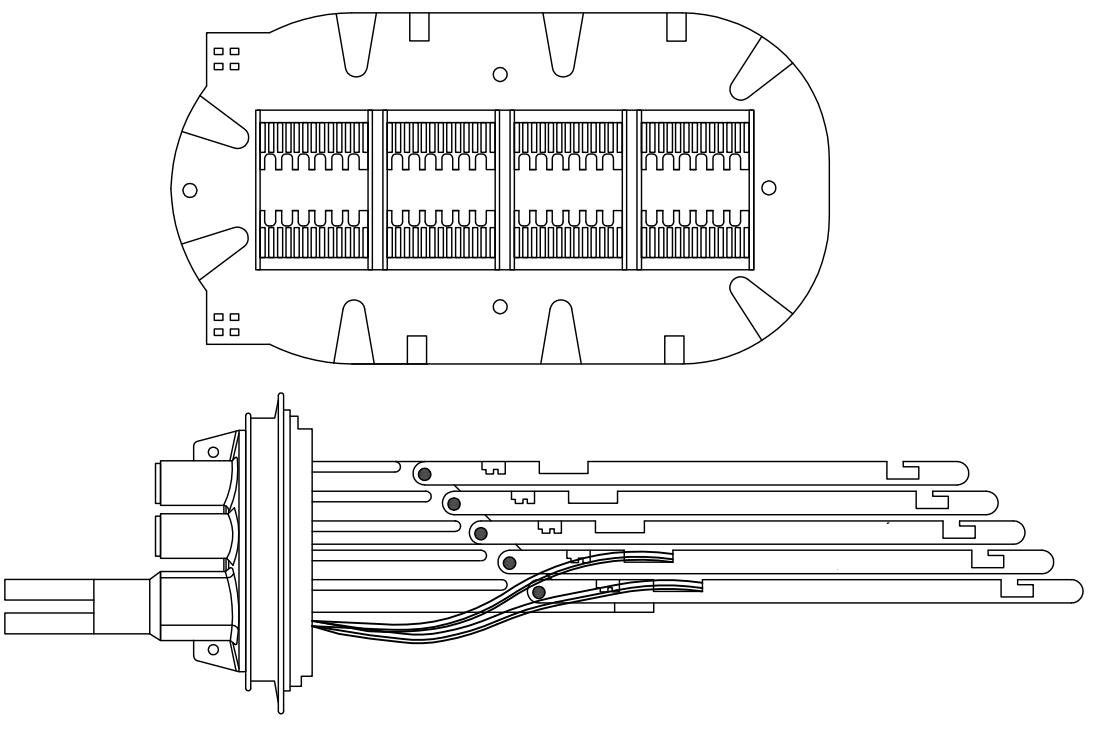
\includegraphics[width=.5\textwidth]{./images/caixa_emenda_detalhe_bandejas.png}
	\caption{Detalhe bandejas em Caixa de Emenda}
	\label{fig:ce_detalhe_bandejas}
\end{figure}

Os cabos ópticos são constituídos de fibras agrupadas em tubos. Cada fibra por
sua vez, pode trafegar zero, um ou vários comprimentos de onda ($\lambda$).
Em uma rede física, as fibras são redirecionadas nos vértices (CEs e CAs) de
acordo com as demandas de atendimento das operadoras. CAs atendem clientes finais,
geralmente com o uso de tecnologias de Redes Ópticas Passivas (PON).

Esse redirecionamento das fibras ocorre com o uso de máquinas de fusão
\cite{maeda2009optical}, onde cada par de fibras é acomodado em bandejas,
conforme mostra a Figura \ref{fig:ce_detalhe_bandejas}. Em um caso ideal,
espera-se que de acordo com as requisições de demanda recebida, a ocupação das
ranhuras seja feita de forma sequencial e organizada. Por exemplo, em um cabo
contendo 12 tubos, com 12 fibras cada cabo, o grupo de ranhuras superior recebe
o primeiro tubo, o segundo grupo o segundo tubo, assim por diante.

\subsection{Algoritmos para Cálculo de Rotas}

Para descobrir a melhor rota, ou seja, qual sequência de cabos e caixas é o
caminho mais curto entre uma caixa A e B, podemos considerar pelo menos dois
algoritmos clássicos: Algoritmo de Dijkstra (encontra o caminho de menor custo
em grafos com pesos não negativos) \cite{dijkstra2022note} e o Algoritmo de
Bellman-Ford (lida com arestas de peso negativo, mas com maior complexidade
temporal).

Embora o Algoritmo de Dijkstra não funcione com custos negativos, podemos
considerá-lo, visto que o custo será igual a distância. Um exemplo de uso pode
ser visto na Figura \ref{fig:dijkastra_graph} em conjunto com a Figura
\ref{fig:dijkastra_table}. Importante destacar que o Algoritmo de Dijkstra não
funciona bem para longas sequências de nós, visto que a lógica do mesmo
necessita navegar até o fim do ramo.

Ainda com os problemas observados com o Algoritmo de Dijkstra, podemos
considerá-lo, pois do ponto de vista de complexidade de tempo, observa-se três
etapas que fazem a base dessa complexidade (1) quando um novo vértice é
empurrado/adicionado à fila de prioridades, (2) quando um vértice com distância
mínima é retirado da fila de prioridade e (3) quando a distância de um vértice
é diminuída na fila de prioridade. Considerando uma estrutura de fila com
lista, empurrar e retirar nós da fila são ambos iguais a $O(V)$, reduzir o nó
também igual a $O(V)$. Portanto, conclui-se que o algoritmo tem uma
complexidade de tempo igual a $O(V^2 + EV)$.

O roteamento de fibras pode ser formulado como um problema de programação
linear inteira \cite{griva2008linear}, onde variáveis binárias indicam se uma
fibra ou enlace é utilizado. Entretanto, tais problemas são NP-difíceis
\cite{artigorwa}, devido à combinação exponencial de caminhos possíveis. Por
isso, heurísticas como Dijkstra são práticas e eficientes em instâncias reais
\cite{mukherjee2020springer}.

\begin{figure}
  \begin{minipage}[c]{0.42\linewidth}
	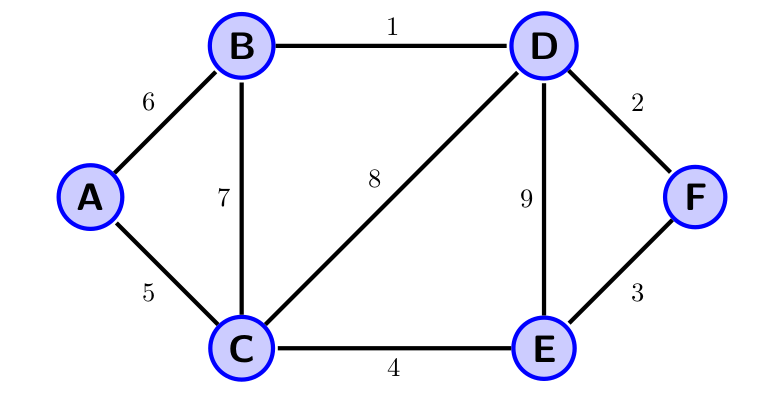
\includegraphics[width=\linewidth]{./images/dijkastra_01.png}
	\caption{Grafo com custos}
	\label{fig:dijkastra_graph}
  \end{minipage}
  \hfill
  \begin{minipage}[c]{0.57\linewidth}
	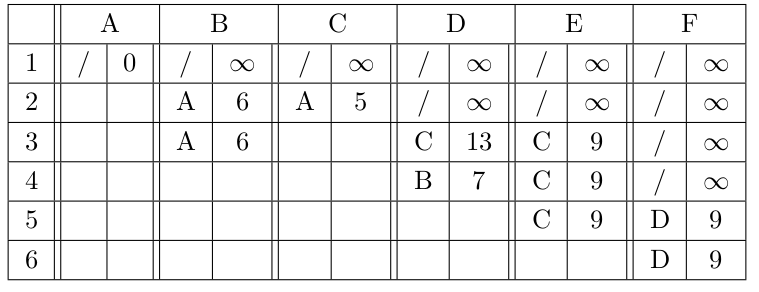
\includegraphics[width=\linewidth]{./images/dijkastra_02.png}
	\caption{Iterações do algoritmo Dijkastra}
	\label{fig:dijkastra_table}
  \end{minipage}
\end{figure}


Além da escolha do caminho, a rede precisa alocar espectro e largura de banda.
O problema de \textit{Routing and Wavelength Assignment} (RWA) é conhecido por
sua complexidade computacional, reforçando a necessidade de algoritmos
heurísticos e aproximativos \cite{artigorwa}.

